% +--------------------------------------------------------------------+
% | Sample Chapter
% |
% | This file provides examples of how to
% | - insert a figure with a caption
% | - construct a table with a caption
% | - create subsections within the chapter
% | - insert a reference to a Figure or Table
% | - make a citation
% +--------------------------------------------------------------------+

\cleardoublepage

% +--------------------------------------------------------------------+
% | Replace "Chapter Title" below with the title of your chapter.  LaTeX
% | will automatically number the chapters.
% +--------------------------------------------------------------------+

\chapter{Introducción}
%\label{ch:chapter1}
\label{makereference}

Cada vez es más frecuente que dispositivos tecnológicos de uso cotidiano, como smartphones o tablets, remplacen a los ordenadores personales, y no sólo en los hogares, sino también en los centros educativos, encontrando profesores que realizan clases utilizando este tipo de dispositivos. La plataforma eAdventure, así como los videojuegos generados por esta plataforma, funcionan sobre la maquina virtual Java, la cual cada vez dispone de menos soporte en este tipo de dispositivos. Por lo que, todos aquellos juegos generados en eAdventure, cada vez están disponibles para menos público, y dado que éstos son en su mayoría videojuegos educativos, con contenido de gran valor para la educación, tanto a nivel estudiantil, como de instrucción, concienciación y formación de trabajadores, es importante facilitar que todo el desarrollo realizado sobre eAdventure se pueda explotar y utilizar en cualquier tipo de plataforma.

Este es el caso del videojuego Checklist, creado en eAdventure para formar a personal sanitario, recalcando la importancia de realizar siempre la Lista de Verificación Quirúrgica. Este videojuego fue desarrollado por el equipo de investigación de eUCM y únicamente cuenta con versiones que se pueden ejecutar sobre Windows, Mac OSX y Linux. Checklist es objeto de el trabajo y se reconstruirá sobre Unity, motor de videojuegos muy popular, caracterizado por la amplia portabilidad de los videojuegos creados con dicho motor.

El planteamiento de la reconstrucción de dicho videojuego, lleva a la evolución de este proyecto en algo reutilizable, generando una herramienta capaz de interpretar el contenido de cualquier juego generado por eAdventure, y permitir jugarlo. Así como la posibilidad de generar dicho juego, en un paquete único ejecutable, y compatible con múltiples plataformas y sistemas operativos.

Gracias a este caso personal y la experiencia portando dicho videojuego, se realizará una explicación acerca de cómo evolucionó este proyecto desde el planteamiento de una reconstrucción de juego, así como sus múltiples iteraciones en el diseño de arquitectura, y su posterior integración junto al proyecto de Piotr Marzsal. En este proceso se exponen todos aquellos problemas que surgen, así como su resolución, enfrentando un cambio de paradigma en el que se pasa de tener una arquitectura orientada a objetos, a una arquitectura orientada a componentes. 


%\begin{figure}[htb]%t=top, b=bottom, h=here
%
%    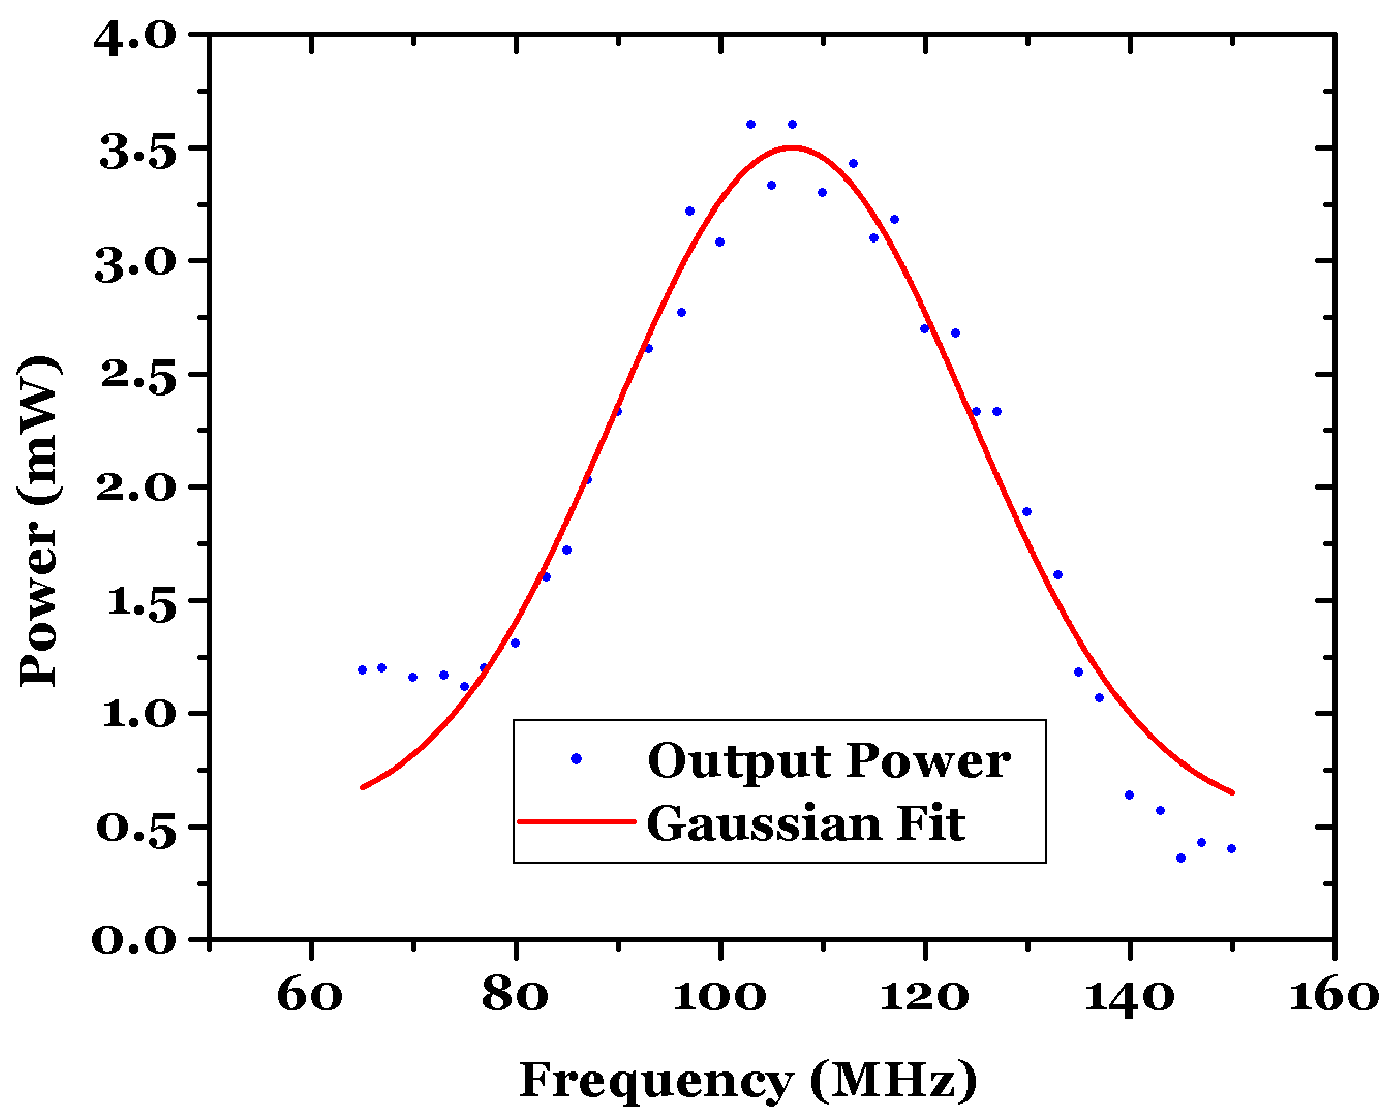
\includegraphics[height=2.5in]{figures/graph.png}
%
%    \caption[Optional: Short caption to appear in List of
%    Figures]{Full caption to appear below the Figure}
%
%    \label{figure1}
%\end{figure}

% +--------------------------------------------------------------------+
% |To create cross-references to figures, tables and segments
% |of text, LaTeX provides the following commands:
% |   \label{marker}
% |   \ref{marker}
% |   \pageref{marker}
% | where {marker} is a unique identifier.
% |
% | In the line above, we use \label{figure1} to mark a location
% | we wish to refer to later.  LATEX replaces \ref by the number of
% | the chapter, section, subsection, figure, or table after which the
% | corresponding \label command was issued. \pageref prints the page
% | number of the page where the \label command occurred.
% |
% +--------------------------------------------------------------------+

%\begin{table}
%
%% +--------------------------------------------------------------------+
%% | We include the command \begin{center} to center the table
%% | horizontally on the page.  Note use of the command \end{center}
%% | to turn off centering after the table is defined.
%% +--------------------------------------------------------------------+
%    \begin{center}
%
%% +--------------------------------------------------------------------+
%% | The table is created with this command
%% |
%% | \begin{tabular}[pos]{table spec}
%% |
%% | The "pos" argument specifies the vertical position of the table relative to
%% | the baseline of the surrounding text.  Use t, b, or c to specify alignment
%% | at the top, bottom, or center.
%% |
%% | The "table spec" command defines the format of the table
%% |   l for a column of left-aligned text
%% |   r for a column of right-aligned text
%% |   c for centered text
%% |   p{width} for a column containing justified text with line breaks
%% |   | for a vertical line
%% +--------------------------------------------------------------------+
%
%    \begin{tabular}[c]{|c|c|c|}
%        \hline
%        Column 1 Heading & Column 2 Heading & Column 3 Heading \\
%        \hline
%        Col 1 Row 1 & Col 2 Row 1 & Col 3 Row 1\\
%        Col 1 Row 2 & Col 2 Row 2 & Col 3 Row 2\\
%        Col 1 Row 3 & Col 2 Row 3 & Col 3 Row 3\\
%        \hline
%    \end{tabular}
%    \caption{Caption to appear below the table}
%    \label{table1}
%   \end{center}
%\end{table}

% +--------------------------------------------------------------------+
% | Replace \section headings below with the title of your
% | subsections.  LaTeX will automatically number the subsections 1.1,
% | 1.2, 1.3, etc.
% +--------------------------------------------------------------------+

\section{Los videojuego educativos y el E-Learning}
\label{seriousgames}

El e-Learning, también conocido en español con la terminología de Aprendizaje Electrónico, es aquello que, según Martín Hernández, engloba aquellas aplicaciones y servicios que, tomando como base las TIC, se orientan a facilitar el proceso de enseñanza-aprendizaje [1]. Este e-Learning surgió en un primer momento con la intención de facilitar el acceso a la información al mayor número de personas posibles, pero esto fue satisfecho rápidamente por sistemas muy simplificados de e-Learning que básicamente son grandes repositorios de información con unas pocas facilidades.

Este sector, sin embargo, está avanzando para que no haya tanta diferencia con los sistemas de educación tradicionales, intentando reducir la separación que se produce entre un profesor y un alumno cuando se realiza la educación mediante plataformas educativas en línea, añadiendo elementos de monitorización y seguimiento, elementos que fomentan la participación en comunidad como foros de trabajo, o añadiendo elementos de gamificación en los proyectos de aprendizaje que se desarrollan.

No obstante, estos sistemas de educación pese a ser mucho más dinámicos, permitiendo que los usuarios marquen su ritmo de aprendizaje, y presentarse con un enfoque diferente, que supone un grado de implicación personal en el que es el usuario el que decide realizar un aprendizaje, y no una imposición social, familiar o incluso personal; no dan la motivación suficiente a muchos estudiantes para continuar con la educación y no abandonarla. Es por ello que otro tipo de género de herramientas de e-Learning surgen, donde la motivación para aprender se adquiere a través del uso de la herramienta, y el aprendizaje suele ser una cualidad implícita que se adquiere por la utilización de la misma. Estos son los videojuegos educativos.

El abandono escolar es uno de los problemas más importantes actualmente. Según Prensky, los estudiantes son nativos digitales, personas capaces de interactuar con ricos dispositivos digitales como ordenadores, dispositivos móviles o videoconsolas. Esto difiere con las metodologías tradicionales de educación, en términos de interacción y contenido [2].

Por todo ello, los videojuegos educativos suponen un tema de estudio y desarrollo muy importante dentro de las diferentes tecnologías de e-Learning.

%In this paragraph, we want to refer to Fig.~\ref{figure1}
%mentioned at the beginning of this chapter.  We also refer to the
%Table~\ref{table1}.

\section{El Objeto de Trabajo}
\label{objetodetrabajo}

El objeto de trabajo de este proyecto se ha dividido en tres aspectos. En primer lugar la plataforma de desarrollo de videojuegos educativos eAdventure, la cual comienza a sufrir problemas de portabilidad debido a estar desarrollada en Java. En segundo lugar el videojuego Checklist, desarrollado en eAdventure y que se utiliza para formar a personal sanitario acerca de la utilización de la Lista de Verificación Quirúrgica. Y en tercer lugar, el motor de videojuegos Unity, que en contraposición a eAdventure, es ampliamente conocido por las facilidades que brinda a los desarrolladores para exportar sus proyectos en multitud de plataformas diferentes.

\subsection{eAdventure}
\label{eadventure}

Sobre eAdventure Los videojuegos educativos, a la hora de ser producidos, tienen tres grandes problemas a los que los productores del videojuego deben enfrentarse. Estos tres problemas son: 

En primer lugar, la dificultad de balancear la parte divertida y la parte educativa del videojuego. El correcto balance de ambos aspectos es necesario para el éxito del videojuego, pues, si los estudiantes no se divierten mientras juegan, lo mas probable es que terminen abandonando el juego, lo que echaría por tierra todo el esfuerzo de creación del videojuego; y por otra parte, si todos los esfuerzos son puestos en hacer la parte divertida del juego, es posible que el impacto educativo del mismo sea demasiado pequeño. Diversos autores como Dickey defienden que, los videojuegos enfocados en la historia, como cuentacuentos digitales, o aventuras gráficas point-and-click, son géneros que se adecuan mucho a las necesidades de los videojuegos educativos.

Las aventuras gráficas son un género conocido dentro del mundo de los videojuegos, con grandes títulos como Monkey Island, The Day of The Tentacle o, la franquicia española, Runaway. Tal es el grado de popularidad que tienen estos videojuegos que existen herramientas específicas para la creación de videojuegos de este género, como Adventure Game Studio, DAGE o Open SLUDGE. Sin embargo, todo este tipo de herramientas, pese a ayudar mucho a producir videojuegos de este género, pero no aportan funcionalidades específicas para los videojuegos educativos. De esta manera, eAdventure, aporta un enfoque específico orientado a los videojuegos educativos. 

En segundo lugar, el desarrollo de videojuegos es uno de los sectores dentro del desarrollo de software que supone un coste muy grande para su desarrollo, llegando a costar varios millones de dólares. En la última década, han surgido varios proyectos de videojuegos educativos cuyo presupuesto supera los cientos de miles de euros [2]. Sin embargo, con herramientas apropiadas que simplificasen el proceso de desarrollo del juego, y que además fuesen de bajo coste, se podría reducir el presupuesto necesario para desarrollar videojuegos educativos. Es por ello que eAdventure se presenta como una alternativa libre y gratuita para simplificar el desarrollo de videojuegos educativos. 

Y finalmente, en tercer lugar, el último problema que tienen los videojuegos, está relacionado con los problemas de distribución de un videojuego una vez que está desarrollado. Es frecuente encontrar que videojuegos están únicamente
disponibles en una plataforma o sistema operativo, por lo que gran cantidad de personas no pueden disfrutar de un videojuego, y por consiguiente, los desarrolladores no consiguen que sus videojuegos no tengan el efecto deseado.

Sin embargo, esta herramienta, como se mencionó en la introducción, está desarrollada en Java, y produce Applets standalone, que, pese a no necesitar ninguna instalación, necesitan de la maquina virtual Java para funcionar. La máquina virtual Java ha gozado de mucha popularidad a lo largo de los años, pero actualmente cada vez cuesta más encontrar dispositivos de uso cotidiano que dispongan de ella. Tanto es así que, sistemas operativos como Android, cuyo lenguaje de programación principal es Java, han construido su propia máquina virtual llamada Dalvik [3], la cual está siendo sustituida actualmente por ART [4], y que reemplaza completamente a la maquina virtual Java para la ejecución de programas desarrollados en dicho lenguaje.

Es por ello que el desarrollo analizado en este artículo se encarga de mejorar la capacidad de eAdventure para la distribución de juegos, desarrollando un intérprete capaz de visualizar un juego creado en eAdventure, en el motor de videojuegos Unity. 

%In this section, we refer back to text mentioned in
%Section~\ref{makereference1.1} on page~\pageref{makereference1.1}.

\subsection{Checklist}
\label{checklist}

Ante la pregunta ¿Que instrumento reduce el ratio de muertes y complicaciones en cirugía en más de un tercio? Pese a que pueda parecer que son los avances tecnológicos, la calidad de la medicina y de los utensilios, o la higiene en los hospitales, esta no es la respuesta. Estos factores han mejorado la medicina, y han logrado que avance hasta el punto de realizar operaciones que antes considerábamos impensables, ayudando a los médicos a detectar problemas mucho antes de que surjan y a monitorizar situaciones peligrosas. Pero es algo mucho mas sencillo lo que ayuda a evitar muertes y complicaciones, y esto es una simple lista que se realiza antes, durante y después de una operación. Esta lista tiene el nombre de Lista de Verificación Quirúrgica [5].

La Lista de Verificación Quirúrgica fue desarrollada por la Organización Mundial de la Salud en 2007 buscando identificar las normas mínimas de aplicación universal. Se construyó mediante el estudio de pacientes, cirujanos, anestesiólogos, enfermeras y expertos en seguridad de los pacientes a lo largo de dos años. En si, la lista está formada por simples comprobaciones que llevan muy poco tiempo de realizar, y no debe ser una carga para el equipo quirúrgico, pues ellos ya tienen una labor muy importante que llevar a cabo.

El videojuego Checklist surge para concienciar y educar acerca de la correcta aplicación de la Lista de Verificación Quirúrgica, mostrando, tanto los beneficios de aplicarla correctamente, como las consecuencias de una mala aplicación. Se desarrolló en la UCM, por el grupo de investigación eUCM junto con la Facultad de Medicina de la UCM, el Hospital Doce de Octubre y el Massachusetts General Hospital [6].

Este juego está desarrollado utilizando eAdventure, y por consiguiente es del género Aventura Gráfica, más concretamente, una en Primera Persona, en la que el jugador no maneja a un personaje dentro de un juego, sino que ocupa el lugar del protagonista, quien toma uno de los diferentes roles que se ofrecen y que participan dentro de un quirófano, y realiza participación en una operación en tres situaciones diferentes: Antes de inducir la anestesia al paciente, antes de la primera incisión en la piel, y antes de que el paciente se marche de la sala de operación. Asimismo, dentro del videojuego suceden diferentes eventos que se dan de forma aleatoria, como una incisión mal marcada, o un compañero que no coopera.

El paquete ejecutable está disponible en Windows, Mac OS X y Linux, en versiones de 32 y 64 bits. Adicionalmente, el Applet Standalone se puede encontrar en el repositorio en Sourceforge de eAdventure, y permite la ejecución mediante el uso de la máquina virtual Java. Sin embargo, la ejecución de dicho juego en Tablets Android e iPad no está disponible, por ello se realiza la adaptación de dicho juego a Unity 

\subsection{El motor de videojuegos Unity}

Los motores de videojuegos son herramientas que permiten y facilitan la creación y desarrollo de un videojuego. Estos, dan la funcionalidad básica de proveer de un entorno gráfico para la representación del videojuego, así como un motor físico con detección de colisiones, junto con un bucle principal que se encarga de procesar y ceder tiempo de procesamiento para cada uno de los elementos del videojuego.

Unity es un motor de videojuegos caracterizado por ser capaz de producir videojuegos para multitud de plataformas, entre las cuales encontramos Windows, OS X y Linux, junto con los mas frecuentes sistemas operativos móviles y de tabletas, como Android e  iOS, tanto iPad como iPhone, además de videoconsolas como PlayStation 3, PlayStation Vita, Wii, Wii U, etc. Esta facilidad para producir videojuegos en múltiples plataformas, así como su licencia gratuita para los desarrolladores independientes, y pequeñas startups que no tienen presupuesto para pagar las costosas licencias de los motores de videojuegos, hacen de este motor una opción muy elegida por gran número de desarrolladores que quieren llegar al mayor número de personas con el menor esfuerzo posible.

Asimismo, otras de las características de este motor incluyen la, ampliamente utilizada en videojuegos, arquitectura basada en componentes, en la que los objetos se componen de distinta manera dependiendo de sus necesidades en cada momento, permitiéndoles mutar o adquirir un comportamiento adicional si se requiere; en contraposición a la arquitectura orientada a objetos, en la que los objetos adquieren una funcionalidad al implementar una interfaz o heredar de una clase de una jerarquía superior, así como adquirir funcionalidad mediante la implementación de si misma. Esta arquitectura permite tener objetos más dinámicos, así como facilitar la reutilización de código gracias a la incorporación del mismo componente en varios objetos, sin embargo supone un cambio de paradigma en la programación, y requiere conocer tanto el funcionamiento de Unity, la comunicación entre sus componentes, así como el complejo ciclo de vida que compone cada Tick de juego [7].

En Unity, cada objeto que toma partido dentro de la escena, está constituido por un GameObject y todas aquellas componentes asociadas, extendiendo a la clase MonoBehabiour, así como una componente Transform que le permite orientarse y deformarse en la escena, y una

\section{Estado del Arte}
\label{estadodelarte}

Una vez hemos definido correctamente el objeto de trabajo de este proyecto, compuesto por todos aquellos elementos que lo forman, se analizarán otras alternativas a los objetos presentados en el anterior apartado. 

Frecuentemente ocurre que no existe una única forma de hacer las cosas, y por ello, existen multitud de herramientas disponibles para el desarrollo de Aventuras Gráficas Point and Click, así como de generación de aplicaciones multiplataforma, motores de videojuegos, y herramientas de learning analytics. Todas estas herramientas, además de ayudar a definir mejor los objetivos del trabajo, buscando generar una herramienta que innove y añada funcionalidad adicional a las existentes, ayudan en el desarrollo del proyecto a contextualizar mejor la aplicación, y a inspirar algunos de los elementos de esta misma aplicación.

\subsection{Herramientas de desarrollo de Aventuras Gráficas}
\label{herramientasaventuras}

Al ser un género tan conocido el de las aventuras gráficas, existen multitud de editores que facilitan la generación de este tipo de juegos. Algunos mas conocidos que otros, con diferentes características y funcionalidades propias. Otros que, desgraciadamente, aunque son conocidos por generar aventuras gráficas de renombre, no son públicos, pero de los cuales podemos, mediante el análisis de dichos juegos, extraer funcionalidades, y casos reales de características que tuvieron éxito.

Dentro de esto de editores, encontramos a el más conocido de todos ellos, Adventure Game Studio, también conocido por sus siglas AGS. Está caracterizado por la increíble personalización que tienen los juegos que se generan con esta herramienta, permitiendo modificar prácticamente todos los elementos que lo conforman, además de dar la oportunidad a los desarrolladores, de generar su propios Scripts e incluirlos en el juego. Este software no sólo es un gran editor que da casi infinitas posibilidades, sino que además está acompañado de una gran comunidad de usuarios, desarrolladores indie y aficionados, que comparten entre ellos sus proyectos. Todos estos proyectos compartidos, son debidamente catalogados en el repositorio de juegos que provee la propia página web de esta herramienta. Una de las pegas que tiene este editor es que únicamente funciona en Windows, aunque existen alternativas muy similares para linux. Finalmente mencionar que este motor, pese a ser gratuito para proyectos que no son comerciales, tiene una licencia que, en caso de ser comercializado, establece que el usuario debe encargarse de pagar por todas las librerías que AGS utiliza para funcionar a los desarrolladores de dichas librerías.

\begin{figure}[htb]
    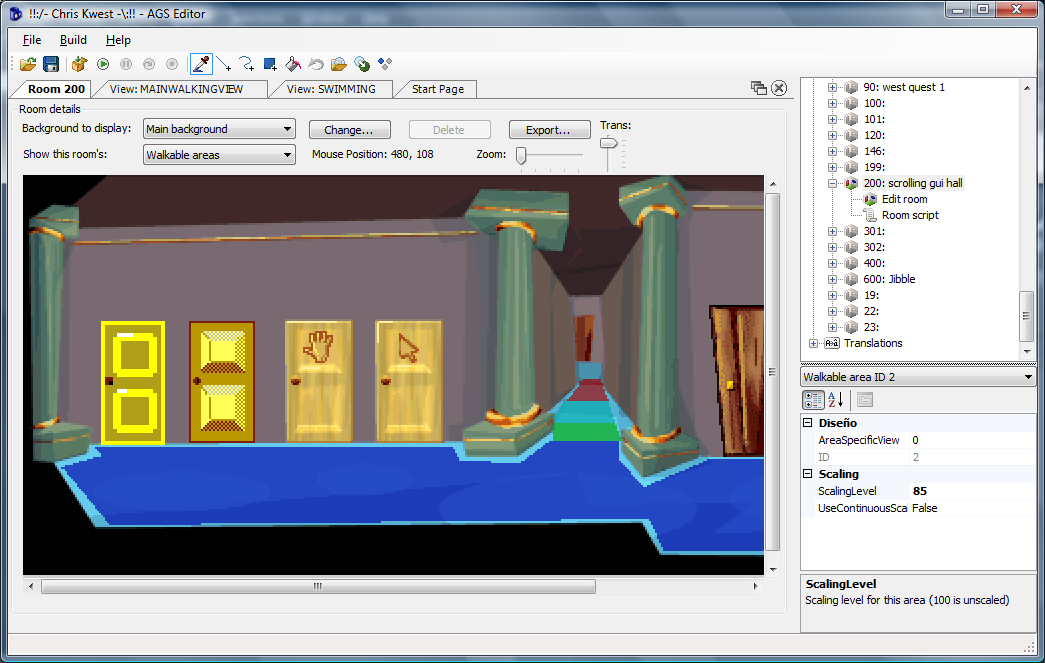
\includegraphics[height=2.5in]{figures/ags.png}
    \caption[Adventure Game Studio]{Una escena en Adventure Game Studio}
    \label{agsfigure}
\end{figure}

En la figura \ref{agsfigure} se puede observar la vista principal del editor, con una escena en la parte del centro-izquierda. En la parte superior derecha se ve la lista de escenas disponibles, y cuando estas se abren, se añaden en forma de pestañas al editor.

Otro de los editores de aventuras gráficas más conocidos es Open SLUDGE. Este editor tiene una enorme lista de características disponibles, entre las cuales encontramos no sólo las básicas como personajes, objetos, escenas, o elementos interactuables; sino que además, encontramos características como poder realizar paralajes en fondos de escenas, que además pueden moverse a lo largo de la escena, posibilidad de añadir música y efectos de sonido, uso de timers, y muchas otras características. No obstante, este editor tiene algunos problemas, como que, por ejemplo, la cámara no sigue al personaje, o no tiene un buen editor de conversaciones, pese a que estas, si que tienen soporte para ser traducidas y localizadas fácilmente. Como detalle adicional de este editor, y característica de las más importantes, es que, es multiplataforma, y no solo se puede ejecutar en Windows, OSX y Linux, sino que además, le da al usuario la posibilidad de generar su juego para estas plataformas, en un paquete individual, con todos los recursos incluidos dentro del mismo.

\begin{figure}[htb]
	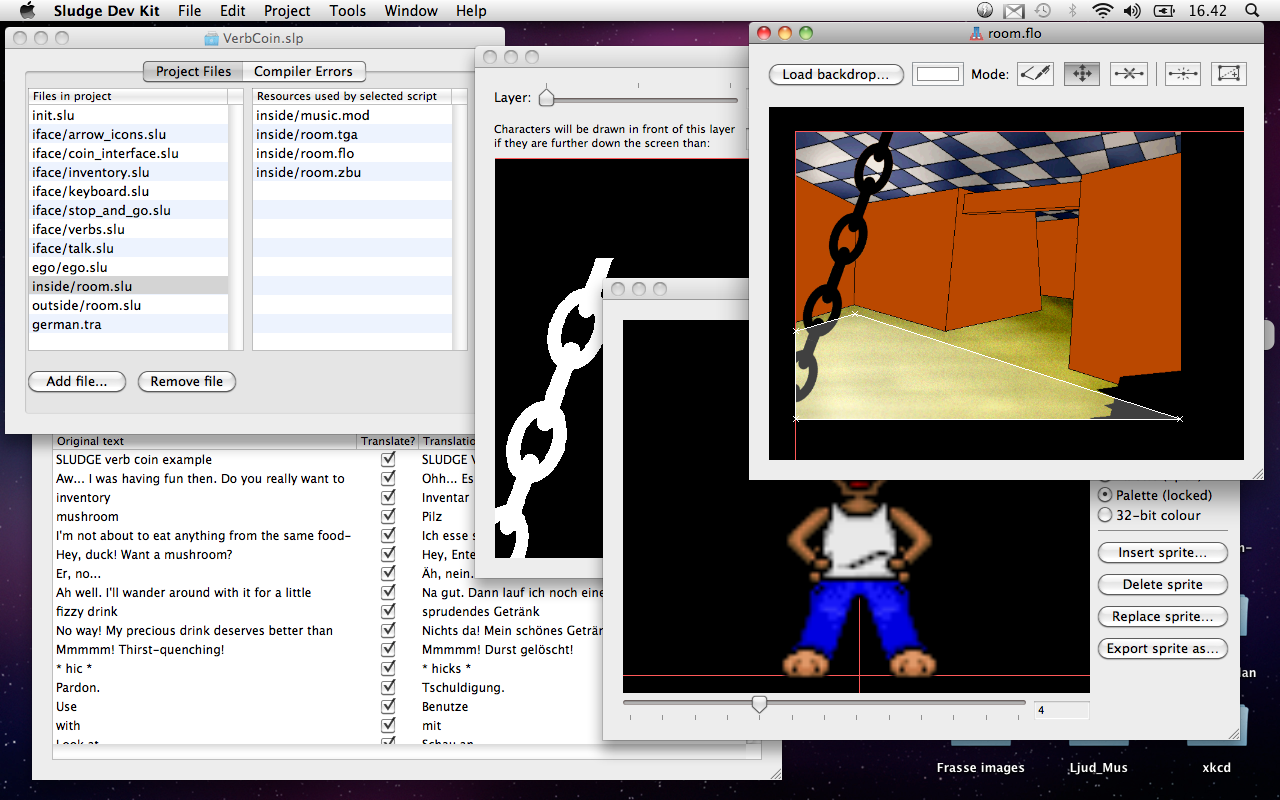
\includegraphics[height=2.5in]{figures/sludge.png}
	\caption[Open SLUDGE]{Multitud de ventanas de Open SLUDGE ejecutándose en OSX}
	\label{sludgefigure}
\end{figure}

En la figura \ref{sludgefigure} se observa como Open SLUDGE se ejecuta en OSX. Las ventanas que se muestran son, por ejemplo, la superior derecha, una previsualización de una escena, con los elementos que hay en ella, y el área dentro de la cual el personaje puede moverse. También, se observa, en el fóndo, un diálogo que está siendo traducido del Inglés al Alemán.

Por último encontramos WinterMute Engine. Este pack de herramientas, cuya primera versión data de enero de 2003, para crear aventuras Point and Click, está caracterizado por ser capaz de crear aventuras gráficas 2D, 2.5D (Personajes en 2 dimensiones, y entornos en 3D, y viceversa), y aventuras generadas completamente en 3D. Al igual que SLUDGE, tiene características estándar como personajes y paralaje en escenas, aunque, frente a este, añade características como editores de interfaz, o soporte a accesibilidad, como poder hacer Text-To-Speech. Sin embargo, una de las características más llamativas de este editor, es la posilibidad de poder generar aventuras gráficas y que estas se ejecuten en iOS, pudiendo instalarlas en un iPad o iPhone. Finalmente decir que el proyecto se distribuye bajo licencia MIT.

\begin{figure}[htb]
	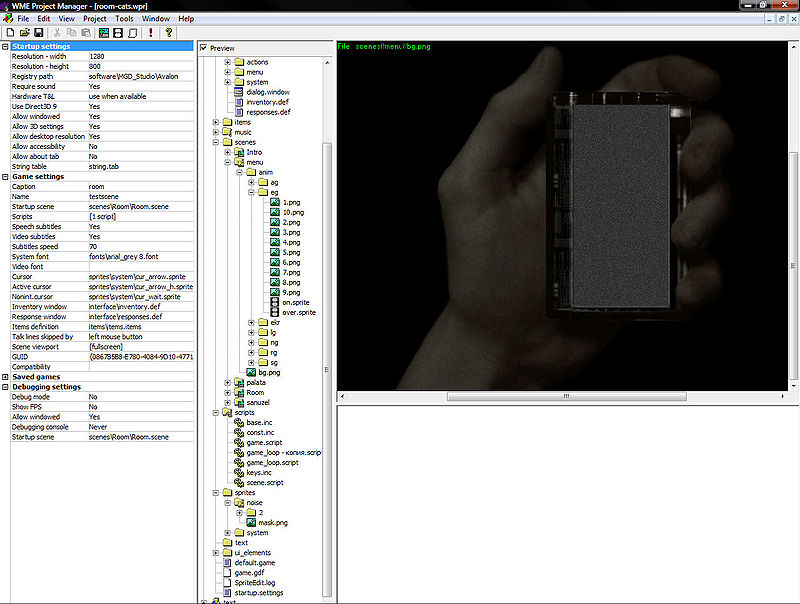
\includegraphics[height=2.5in]{figures/wme.jpg}
	\caption[WinterMute Engine]{Gestor de proyectos de Wintermute Engine}
	\label{wmengine}
\end{figure}

en la figura \ref{wmengine} se muestra una vista del editor WinterMute Engine. La columna central muestra un explorador de archivos que conforman el proyecto, con imágenes y sprites, junto a scripts o otro tipo de archivos. La columna de la izquierda permite configurar el proyecto, y editar características del juego como la resolución del mismo. Y finalmente, la coluna de la derecha es una previsualización del archivo seleccionado.

\section{Metodología de desarrollo}
\label{metodologiadedesarrollo}

Una parte crucial de todo proyecto de ingeniería del software es la metodología de desarrollo que se ha utilizado para su construcción. La metodología determina el proceso de generación del software, pudiendo ser una metodología más lineal como el Proceso Unificado de Desarrollo de Software, o un desarrollo en Cascada, o metodologías basadas en la iteración, como el modelo en espiral de Boehm, o un desarrollo incremetal. Sin embargo, la mayor parte de estas metodologías están pensadas para coordinar a grandes equipos en procesos de desarrollo de larga duración. Por consiguiente, existen metodologías de desarrollo más apropiadas para pequeños equipos que, debido a su configuración de personal y a la rápida comunicación entre miembros, entre otros factores, consiguen que el desarrollo de dicho software sea mucho más ágil.

Asimismo, este proyecto, como muchos de los Trabajos de Fin de Máster, consta de una amplia parte dedicada a la investigación, aprendizaje de nuevas tecnologías, o del desarrollo de prototipos para verificar si esa es la manera más apropiada de hacerlo.

Es por ello que, para desarrollar este proyecto se ha utilizado una metodología de desarrollo ágil, basada en prototipos, en la que se realizan múltiples iteraciones, sobre cada uno de los componentes que conforman el sistema, así como sobre el sistema en sí mismo, realizando tres grandes iteraciones sobre el mismo: 

\begin{itemize}
	\item 
	Una primera iteración para estudiar y analizar los videojuegos de eAdventure, así como para interpretar dichos paquetes e intentar representarlos, aprendiendo de los resultados obtenidos mediante el primer prototipo. 
	\item
	Una segunda iteración generando un mejor diseño de la aplicación, nuevas interfaces, refactorización de clases y código replicado, así como mejoras gráficas visuales dentro de la aplicación.
	\item
	Una tercera iteración, que consiste en poner en funcionamiento el proyecto, separando el proyecto en dos ramas. La primera, en la que se genera un emulador capaz de importar juegos de eAdventure, y permitir al usuario jugarlos, y una segunda que integrando el proyecto de Piotr Marszal junto al intérprete de juegos, transformando ambos proyectos en una única herramienta capaz de generar juegos dentro de Unity. En esta iteración no sólo se generan estos dos proyectos, sino que, como parte del proceso de integración, se adaptan algunas de las clases, eliminando clases que cumplen con la misma función, y reconstruyendo algunos de los elementos para que sean capaces de trabajar en múltiples condiciones.
\end{itemize}

Estas tres iteraciones hacen al proyecto evolucionar desde el primer experimento de "hacer funcionar un juego de eAdventure en Unity" a "generar un framework completo de creación, interpretación, y ejecución de aventuras point and click basado en eAdventure". 

Para dar soporte a la metodología de desarrollo, con mayor frecuencia en la última iteración del desarrollo, se realizaban reuniones periódicas de revisión, generación de tareas para la próxima reunión. Estas reuniones tenían lugar cada 1 o 2 semanas, y estaban formadas por todos los integrantes del desarrollo de ambos proyectos, Baltasar Fernandez Manjón, Iván Martínez Ortiz, Piotr Marszal e Iván José Pérez Colado. Gracias a estas reuniones, la comunicación entre los integrantes ha sido mucho más fluida.